\chapter{Desenvolvimento}
  \section{Requisitos}
  Para Sommerville requisitos de um sistema podem ser entendidos como sendo as descrições do que um sistema deve fazer, os sistemas que ele deve prover [SOMMERVILLE]. Estes requisitos refletem a necessidade do cliente para um sistema que serve a um propósito específico. Este conceito abrange não somente à requisitos de software mas a requisitos de produto também. Neste caso por não existir um cliente real, os requisitos foram levantados juntamente com os idealizadores do produto que são os próprios alunos. 
  Na tabela [REF TABELA] são elicitados os principais requisitos do produto "Bicicleta Elétrica com Dispositivo de Auxílio à Rota"
  
  
  
  \section{Software}
	\subsection{Aplicativo}
	
	\subsection{Comunicação APP e Microcontrolador}
	  A comunicação entre o celular e o microcontrolador será feita através de receptor \textit{bluetooth} acoplado ao microcontrolador. Para que seja feita essa comunicação, será utilizada a API do próprio sistema android para troca de informações via \textit{bluetooth}. Dentre os principais recursos que a API fornece, os que mais serão utilizados serão:
	  \begin{itemize}
	  	\item Busca por outros aparelhos \textit{bluetooth};
	  	\item Pareamento entre o adaptador \textit{bluetooth} e o dispositivo\textit{bluetooth};
	  	\item Conexão com \textit{sockets} específicos de outros aparelhos;
	  	\item Transferência de arquivos;
	  \end{itemize}
	  
	  Deve-se ressaltar que para a utilização do \textit{bluetooth} do aparelho é necessário que o dispositivo permita a utilização de tais recursos, sem essa permissão não é possível fazer a comunicação entre os dois dispositivos.  
  	Para realizar a busca do adaptador \textit{bluetooth} que estará instalado na placa microcontroladora será utilizado o seguinte trecho de código apresentado na figura \ref{img:bluetooth_enabled}
  	
  	\graphicspath{{figuras/}}
  	\begin{figure}[h!]
  	\centering
  	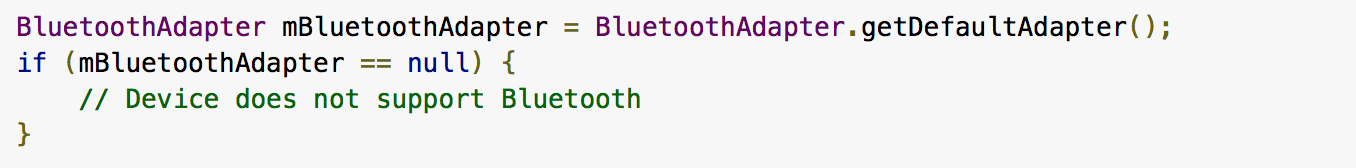
\includegraphics[scale=0.60]{bluetooth_enabled}
  	\caption{Trecho de código exemplificando a comunicação \textit{bluetooth}}
  	\label{img:bluetooth_enabled}
  	\end{figure}
  	
  	Para garantir que o dispositivo \textit{bluetooth} será adicionado apenas uma vez, será utilzado um trecho de código parecido com o da figura \ref{img:bluetooth_devices}, que garante que para um dispositivo ser adicionado ele, não deve estar presente na lista de dispositivos previamente adicionados.
  	
  	\graphicspath{{figuras/}}
  	\begin{figure}[h]
  	\centering
  	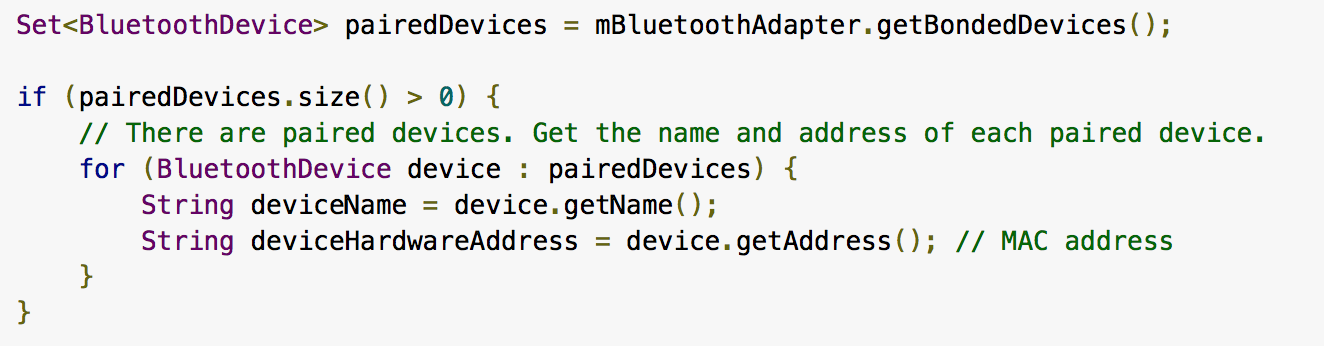
\includegraphics[scale=0.60]{bluetooth_paired_devices}
  	\caption{Trecho de Código que garante que um dispositivo será adicionado apenas uma vez}
  	\label{img:bluetooth_devices}
  	\end{figure}
  	
  	Para que seja feita a transferência de dados entre os dispositivos, o Google (empresa responsável pela documentação da plataforma android), dispõe um trecho de código que serve como guia para implementação desta funcionalidade. Na figura \ref{img:trecho1} é criada uma classe que define as constantes que serão utilizadas ao longo do código.
  	
  	\graphicspath{{figuras/}}
  	\begin{figure}[h!]
  	\centering
  	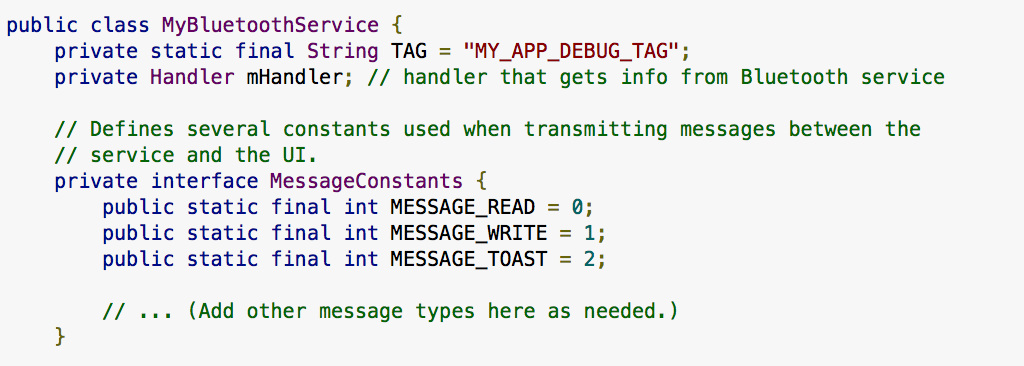
\includegraphics[scale=0.60]{classe_MyBluetoothService}
  	\caption{Neste trecho de código são definidas as constantes que serão utilizadas ao longo do código}
  	\label{img:trecho1}
  	\end{figure}
  
Na figura \ref{img:trecho2} é criada uma outra classe que é a classe que implementa a funcionalidade de troca de dados. Esta classe extende da classe Thread, seus atributos são do tipo \textit{BluetoothSocket}, \textit{InputStream}, \textit{OutputStream} e um \textit{array} de \textit{byte}.

\graphicspath{{figuras/}}
\begin{figure}[h!]
\centering
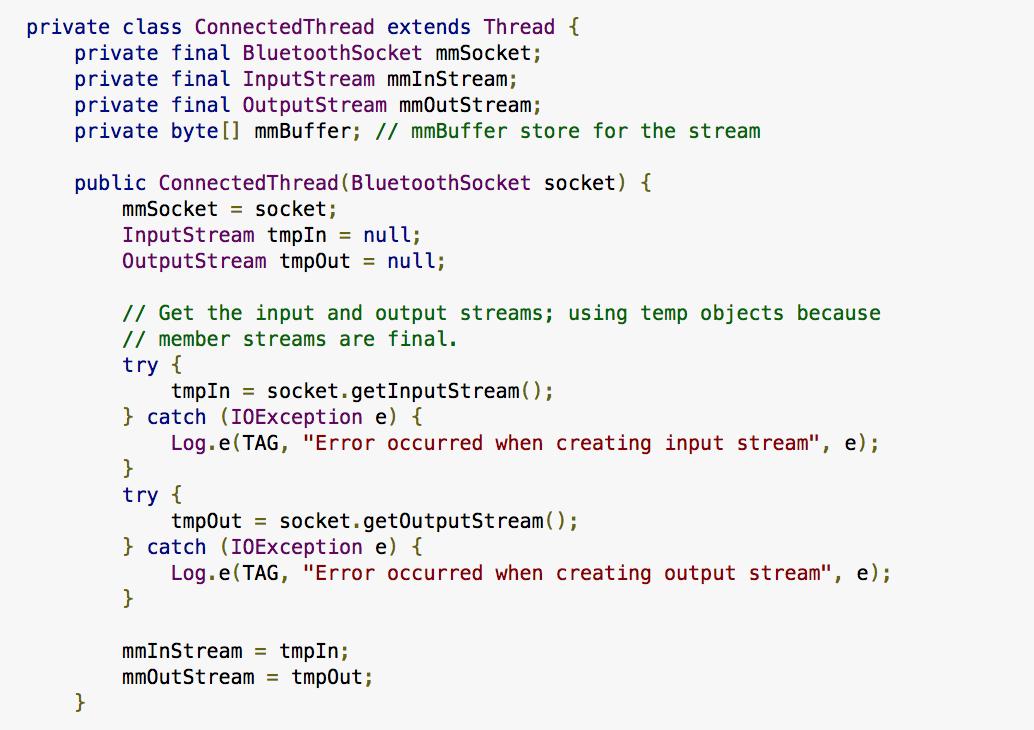
\includegraphics[scale=0.80]{classe_ConnectedThread}
\caption{Nesta classe são implementados os métodos responsáveis pelo funcionamento da troca de dados}
\label{img:trecho2}
\end{figure}

A figura \ref{img:trecho3} apresenta o método \textit{"run"} que funciona em segundo plano constantemente. Este método é responsável por ficar aguardando uma requisição do dispositivo.

\graphicspath{{figuras/}}
\begin{figure}[h!]
\centering
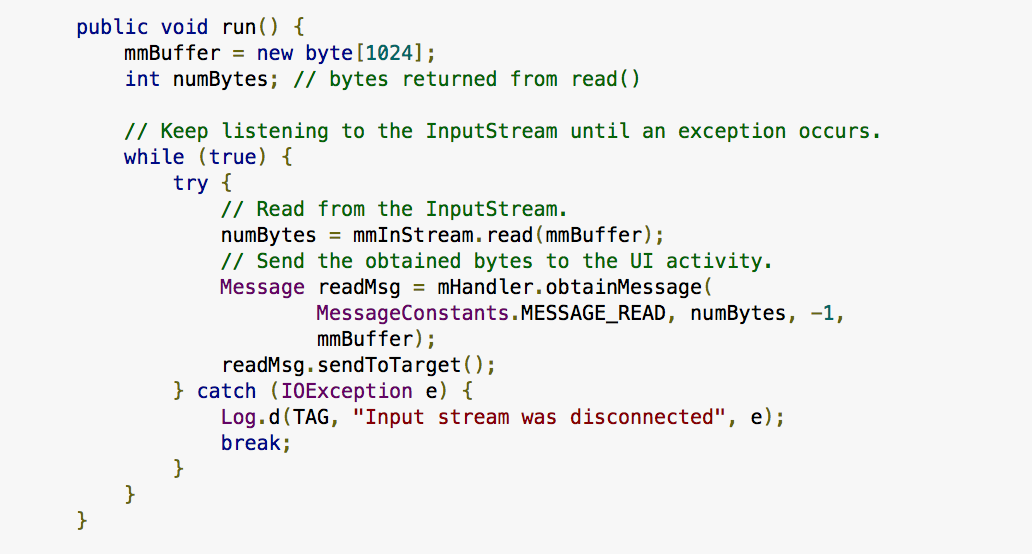
\includegraphics[scale=0.80]{run_method}
\caption{Implementação do método \textit{run} que é responsável por receber as informações do dispositivo \textit{bluetooth}}
\label{img:trecho3}
\end{figure}

O método \textit{"write"} é que faz a escrita dos dados que serão enviados para o dispositivo, como pode ser visto na figura \ref{img:trecho4}.

\graphicspath{{figuras/}}
\begin{figure}[h]
\centering
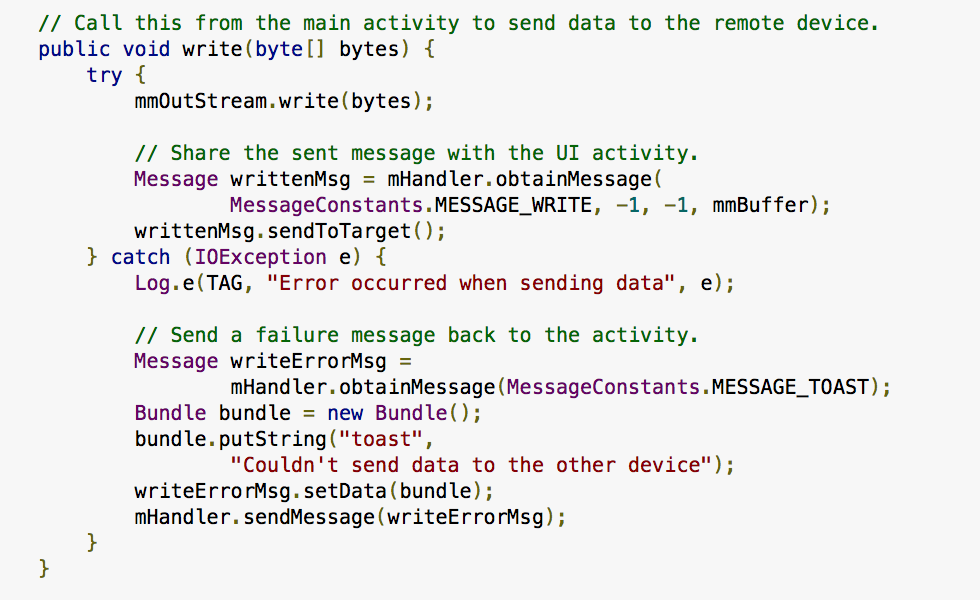
\includegraphics[scale=0.80]{write_method}
\caption{Implementação do método \textit{write} que é responsável por escrever os dados que serão enviados}
\label{img:trecho4}
\end{figure}

Por último, o método \textit{"cancel"} que encerra a conexão com o dispositivo pareado, como mostrado na figura \ref{img:trecho5}

\graphicspath{{figuras/}}
  \begin{figure}[h]
  \centering
  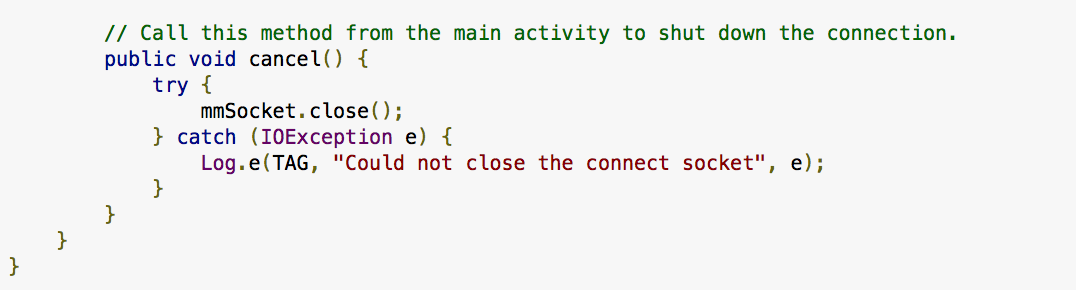
\includegraphics[scale=0.80]{cancel_method}
  \caption{Método \textit{"cancel"} que encerra a conexão com o dispositivo}
  \label{img:trecho5}
  \end{figure}  
  
  \section{Eletroeletrônica}
  	\subsection{Acionamento do Motor}
  
 	 \subsection{Sistema de Controle}
  
  \section{Alimentação}
  
  \section{Estrutura}
  Este projeto visa a construção de uma bicicleta elétrica capaz de seguir uma rota pré-determinada via gps. Porém, há a necessidade de se projetar com a devida atenção toda a estrutura da bicicleta de modo que os demais componentes sejam devidamente adaptados de forma ergonômica, em outras palavras, maximizar a segurança e eficiência da interação máquina e ser humano.
Foram levados em consideração vários fatores, como o material, a estabilidade, conforto e custo-benefício para a escolha e dimensionamento da estrutura.O quadro da bicicleta guardará os motores, baterias e demais componentes eletroeletrônicos de forma segura e organizada. Haverá também, um painel bastante intuitivo que auxiliará o usuário em sua rota como: indicação da bateria restante, distância percorrida e distância restante.
	
	\subsection{Materiais}
	Dentre os materiais que compõem o quadro da bicicleta, foi se escolhido o alumínio, por se tratar de um material leve, barato, com ponto de fusão suficientemente seguro para ser integrado com os componentes eletroeletrônicos além da pouca oxidação sofrida. Outros materiais que foram pesquisados com a finalidade de implementação, foram o aço, porém possui um peso elevado se comparado ao alumínio, e está sujeito a oxidação, apesar do baixo preço. Fibra de carbono, possui um baixo peso, porém um alto custo e uma grande dificuldade na parte de manutenção e conserto.
	
	\subsection{Ergonomia}
	Atualmente no mercado brasileiro as bicicletas mais vendidas são as Mountain Bike, comumente apelidadas de MTB. Isso se deve a sua versatilidade que permite ser utilizada em qualquer terreno. Elas geralmente são encontradas nos tamanho de quadro 17, 18 e 19”. Os dois primeiros tipos são indicados para pessoas entre 1,68 e 1,78 metros de altura enquanto a última atende a faixa de 1,78 e 1,85 metros. 
Segundo a pesquisa de orçamentos familiares realizada pelo IBGE entre 2008 e 2009, a estatura média da mulher e do homem brasileiro adulto são, respectivamente, 1,71 e 1,60 metros. Associando esse dado com os tamanhos de quadros mais comuns do mercado optou-se por utilizar como base para o projeto um quadro de 17”.  
As análises ergonômicas serão realizadas com o auxílio do software CATIA V5 utilizando sua base de dados referente ao estudo de percentil do norte americano. Para o problema apresentado serão adotadas as medidas dos homens de percentil entre 13 e 65, e para mulheres entre 79 e 99, ambos norte americanos.

	\subsection{Design}
	\graphicspath{{figuras/}}
	\begin{figure}[h!]
	\centering
	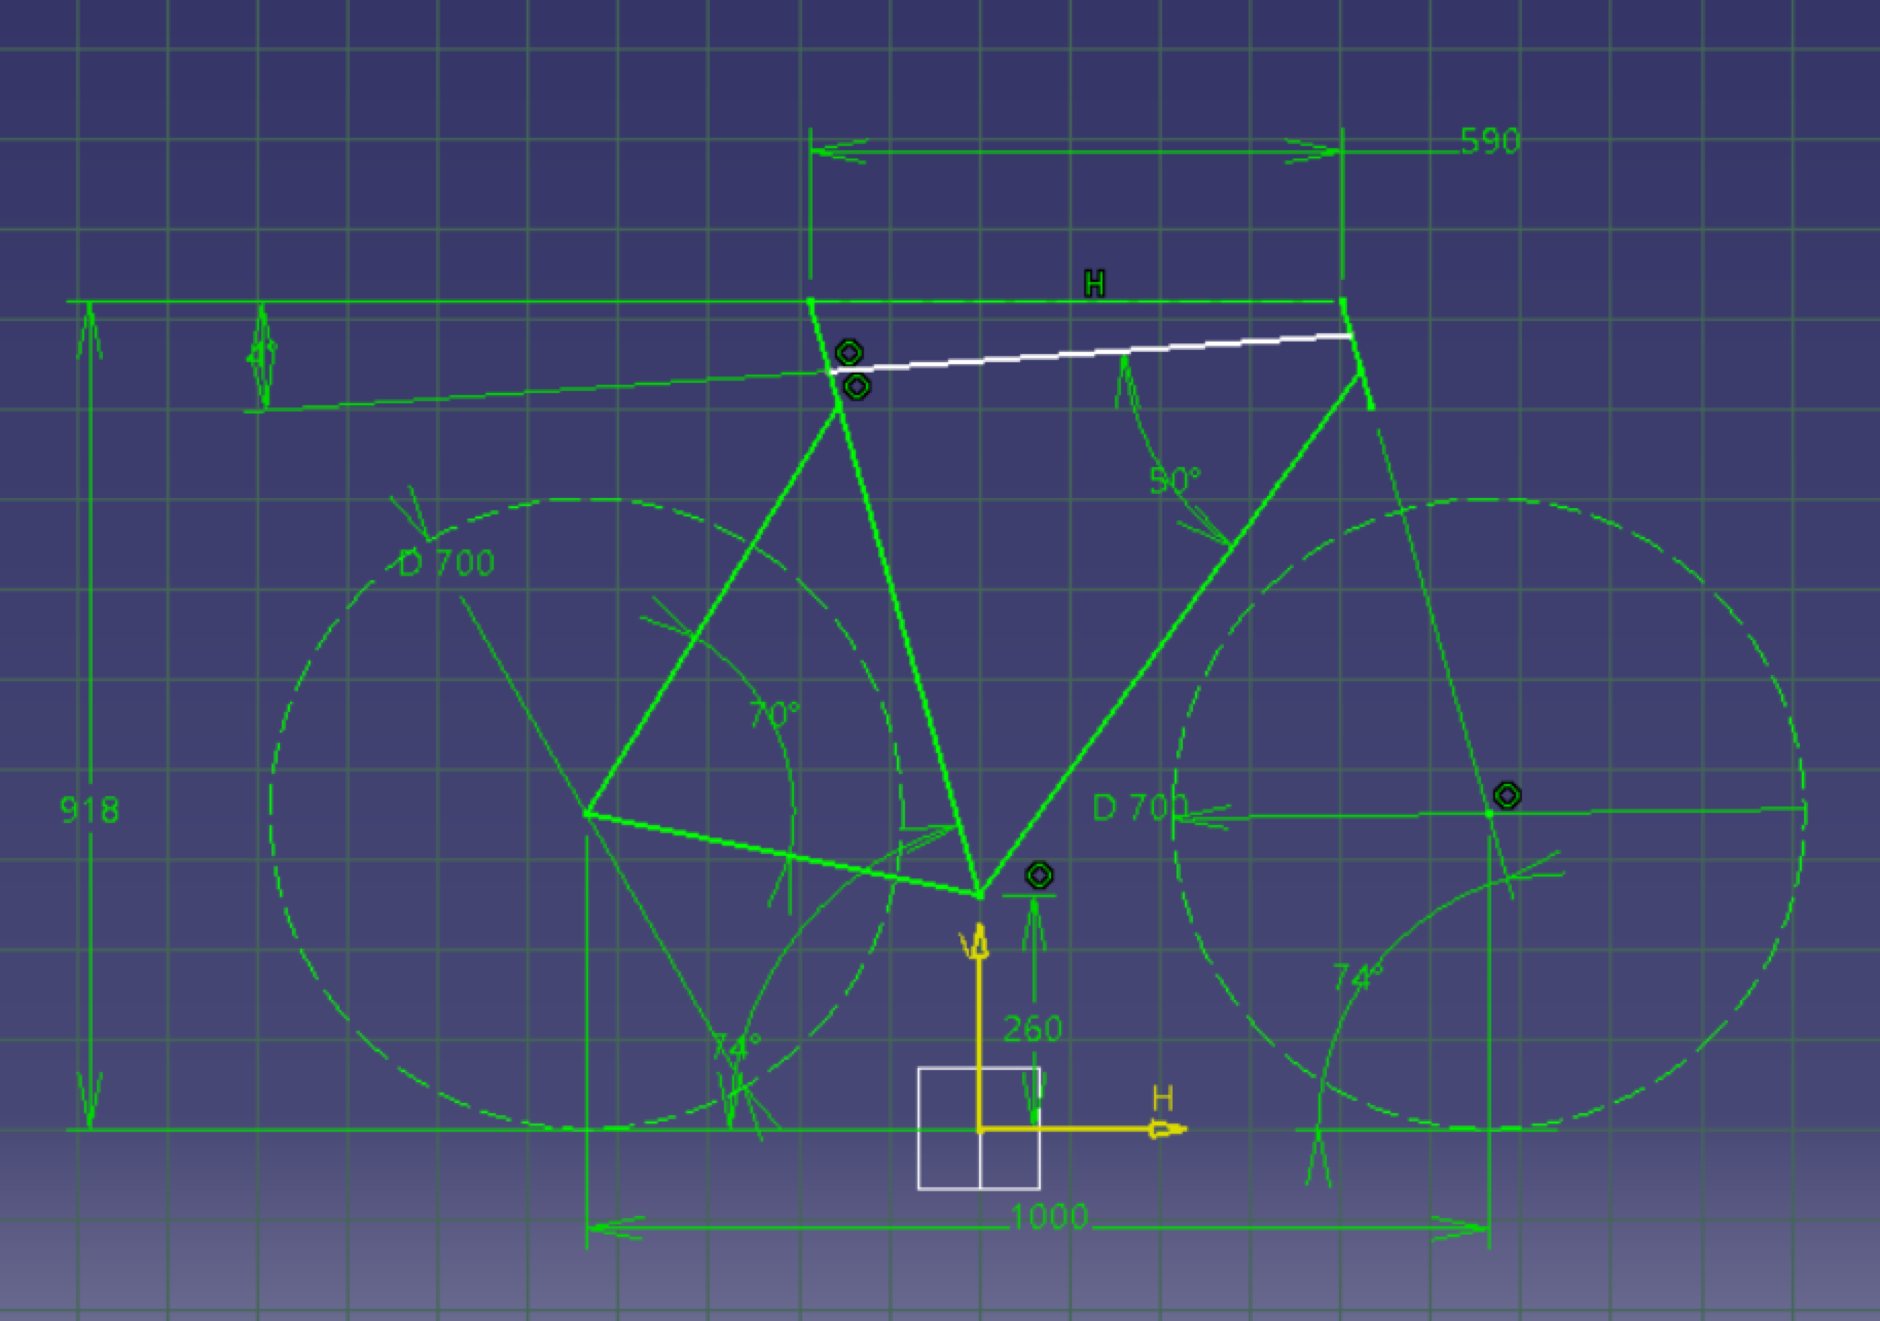
\includegraphics[scale=0.80]{dimensoes.png}
	\caption{Dimensões}
	\label{img:dimensoes}
	\end{figure}


	\subsection{Estabilidade}
	O centro de massa da bicicleta sem os componentes se concentrou em 0,6m no eixo x e 0,5m no eixo y, as forças normais nos pneus traseiros e dianteiros foram de,respectivamente: 24,525N e 73,575N, enquanto as forças de fricção(atrito)  nos pneus traseiros e dianteiros de,respectivamente: 14,96N e 44,88N.

\graphicspath{{figuras/}}
\begin{figure}[h!]
\centering
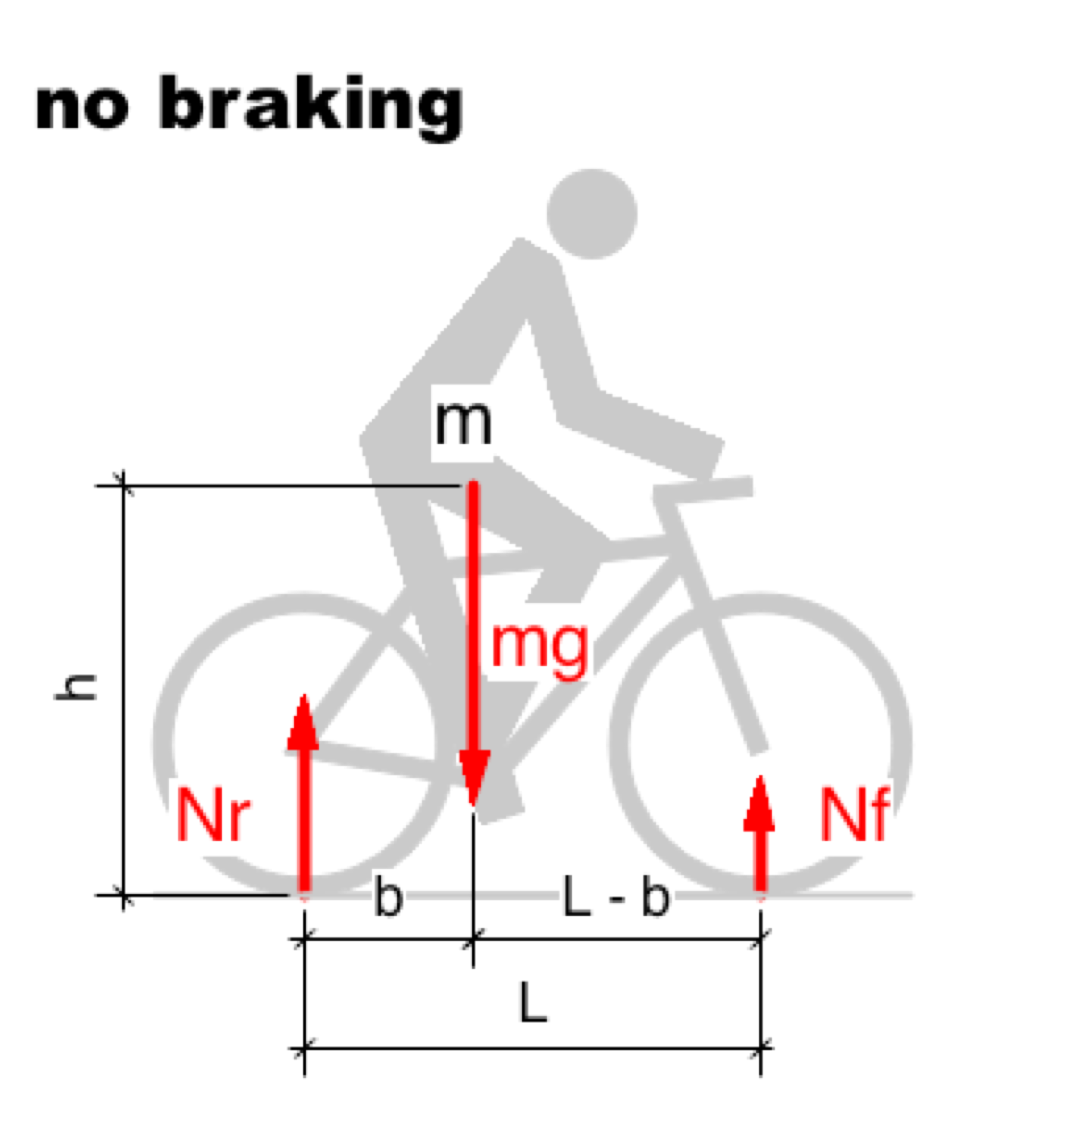
\includegraphics[scale=0.80]{esq_forca_sem_frenagem.png}
\caption{Esquemático de força sem frenagem}
\label{img:esq_forca_sem_frenagem}
\end{figure}

\graphicspath{{figuras/}}
\begin{figure}[h!]
\centering
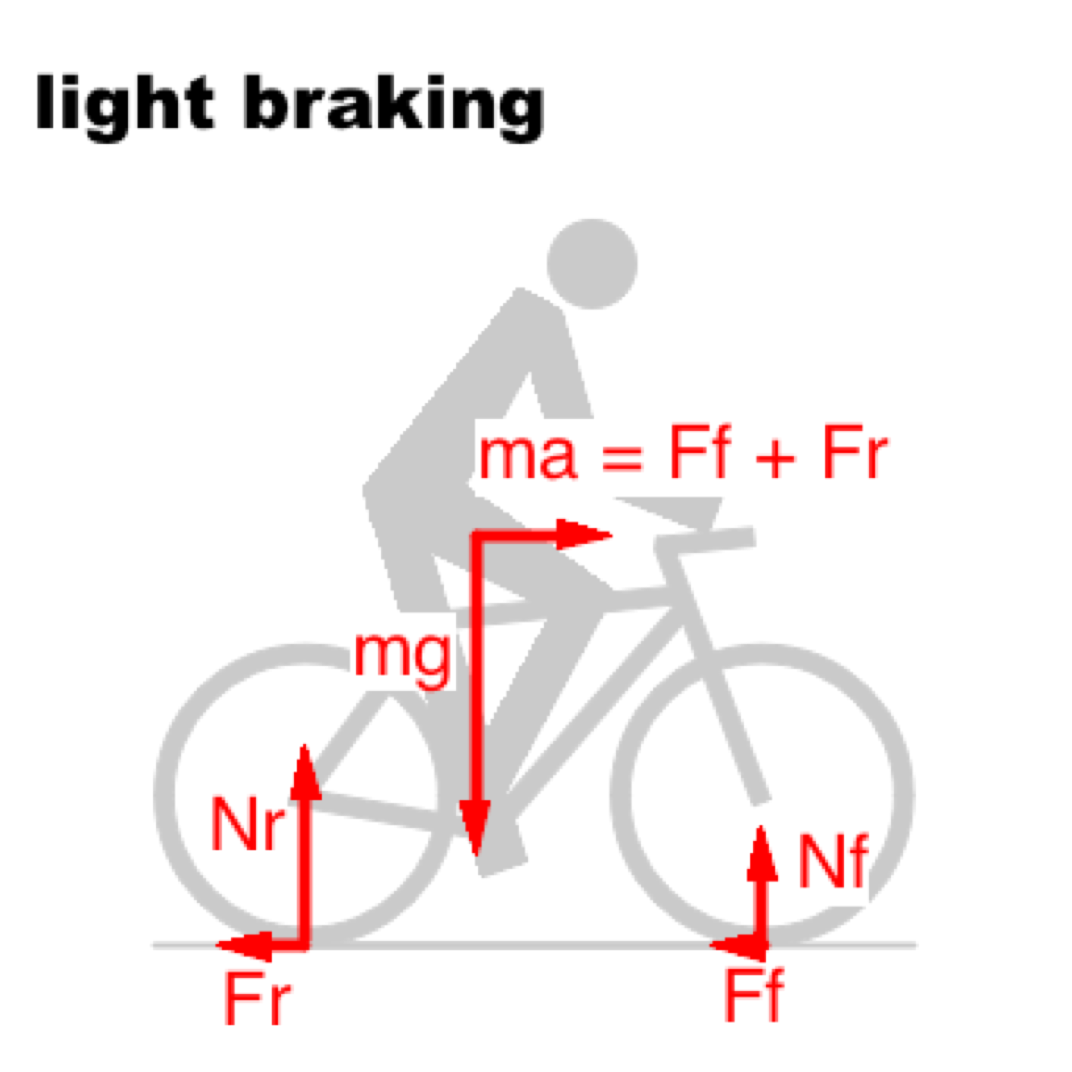
\includegraphics[scale=0.80]{esq_forca_com_frenagem_suave.png}
\caption{Esquemático de força com frenagem suave}
\label{img:esq_forca_com_frenagem_suave}
\end{figure}

\graphicspath{{figuras/}}
\begin{figure}[h!]
\centering
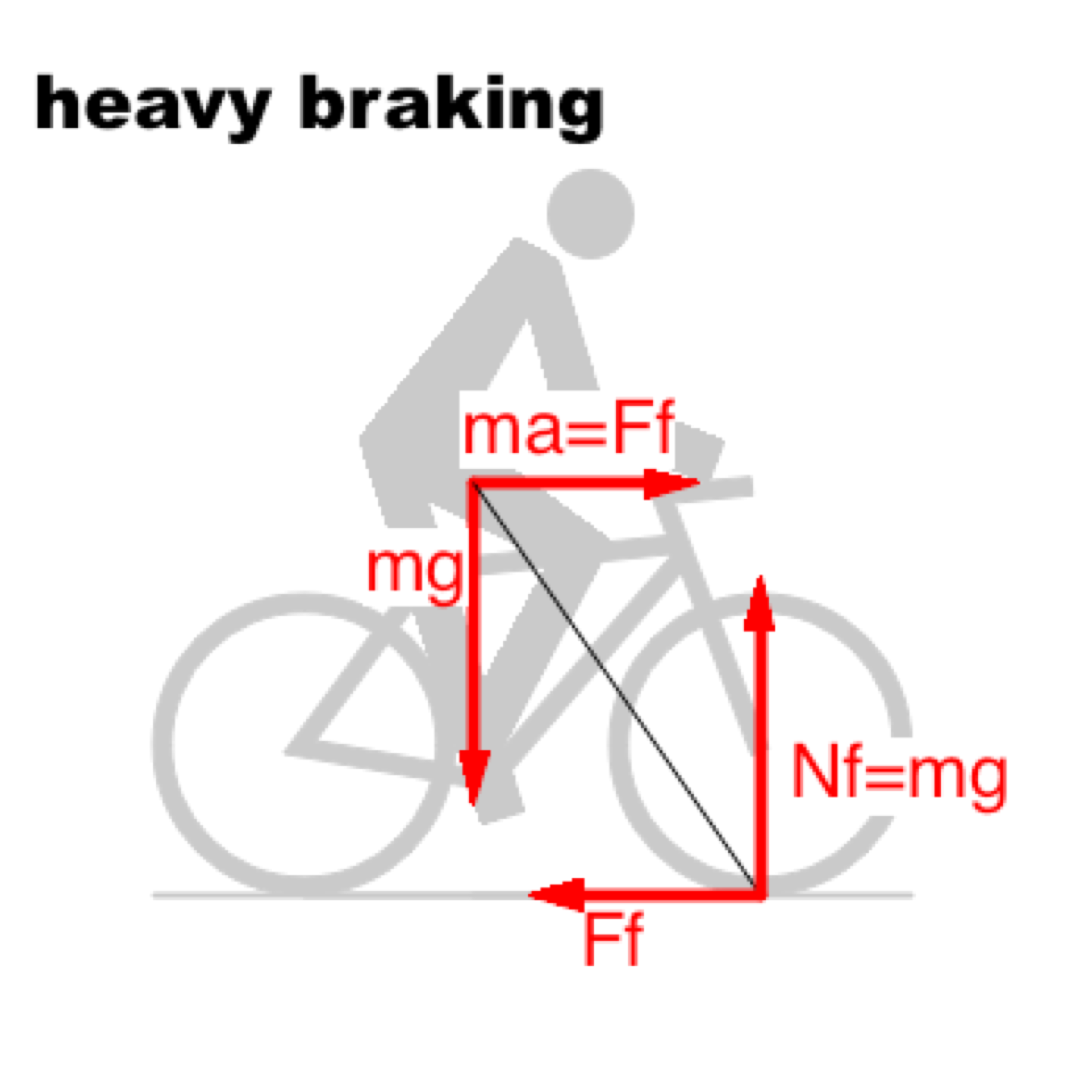
\includegraphics[scale=0.80]{esq_forca_com_frenagem_brusca.png}
\caption{Esquemático de forca com frenagem brusca}
\label{img:esq_forca_com_frenagem_brusca}
\end{figure}


	\subsection{Análises}
	%Foram feitas algumas análises em um quadro de 17 com ajuda dos softwares​ CATIA V5 e Ansys R17.0 no intuito de levantar questões sobre requisitos e melhorias que deverão estar presentes na estrutura.
	
	\subsection{Estática}
	
\graphicspath{{figuras/}}
	\begin{figure}[h!]
	\centering
	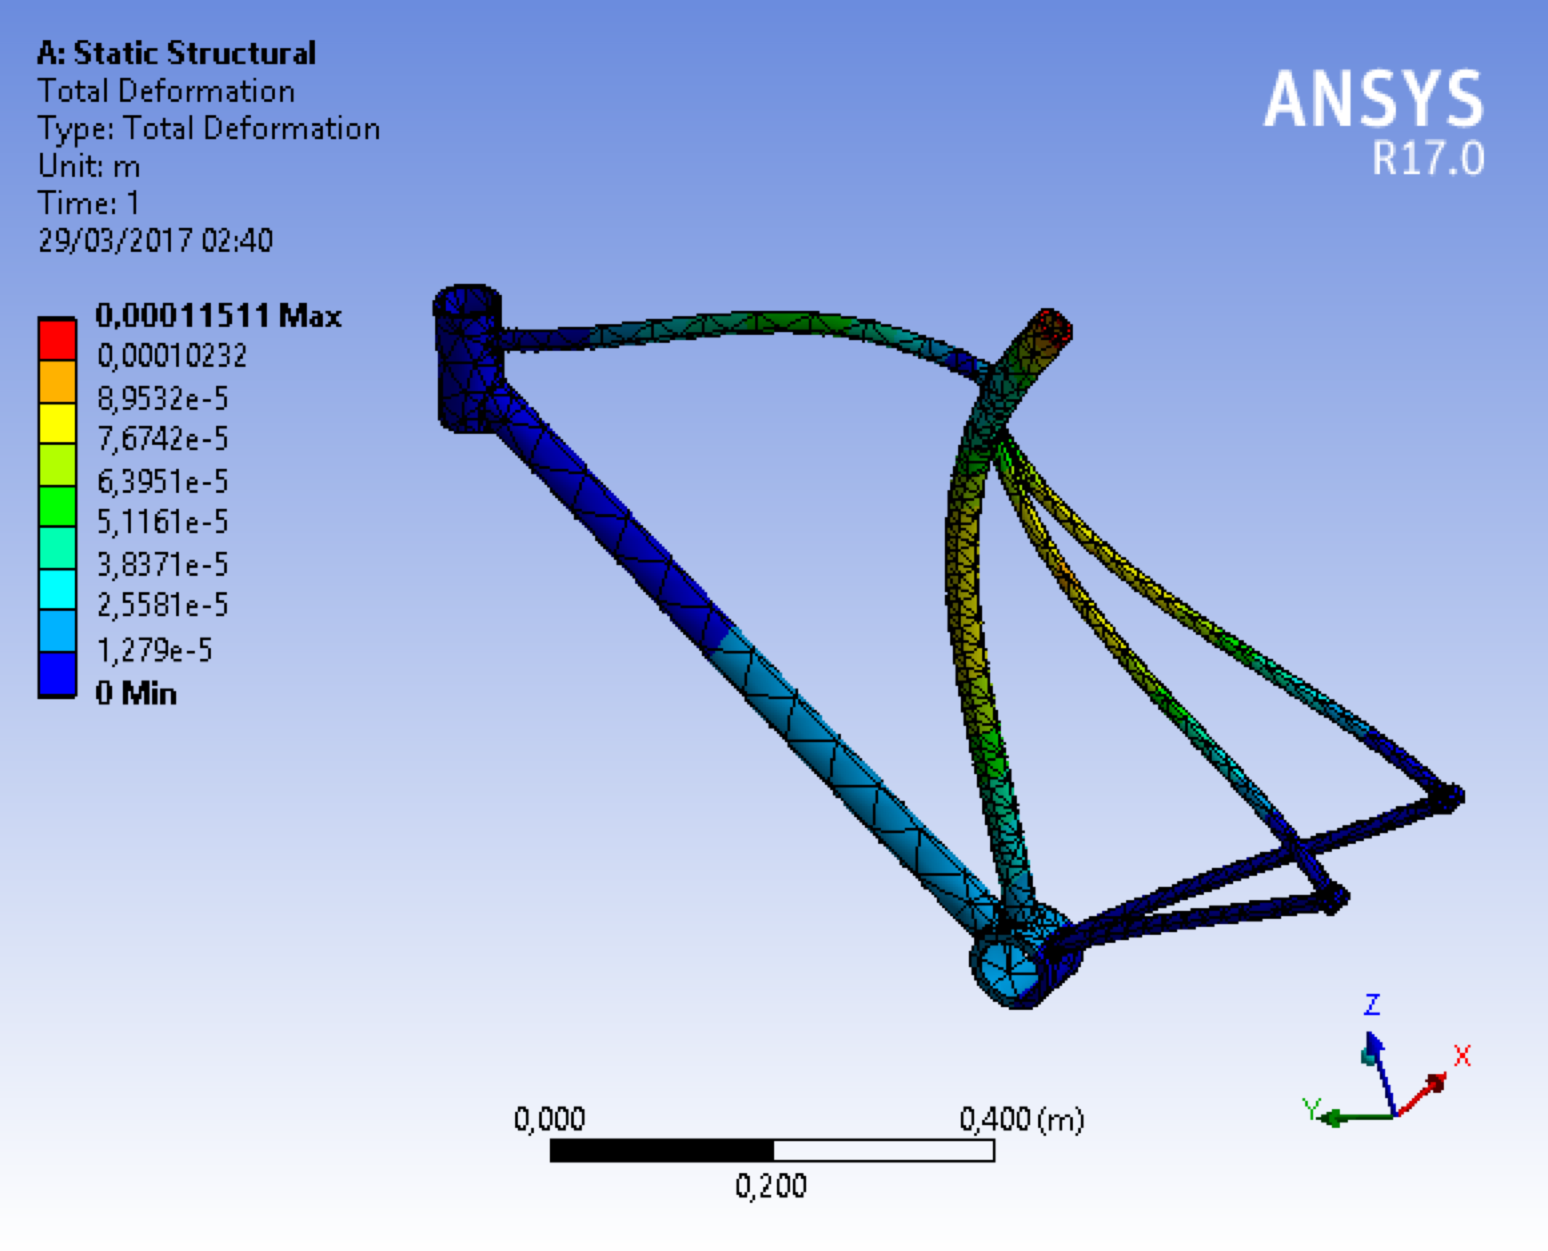
\includegraphics[scale=0.80]{deformacao_total.png}
	\caption{Deformacao total}
	\label{img:deformacao_total}
	\end{figure}	
	
\graphicspath{{figuras/}}
	\begin{figure}[h!]
	\centering
	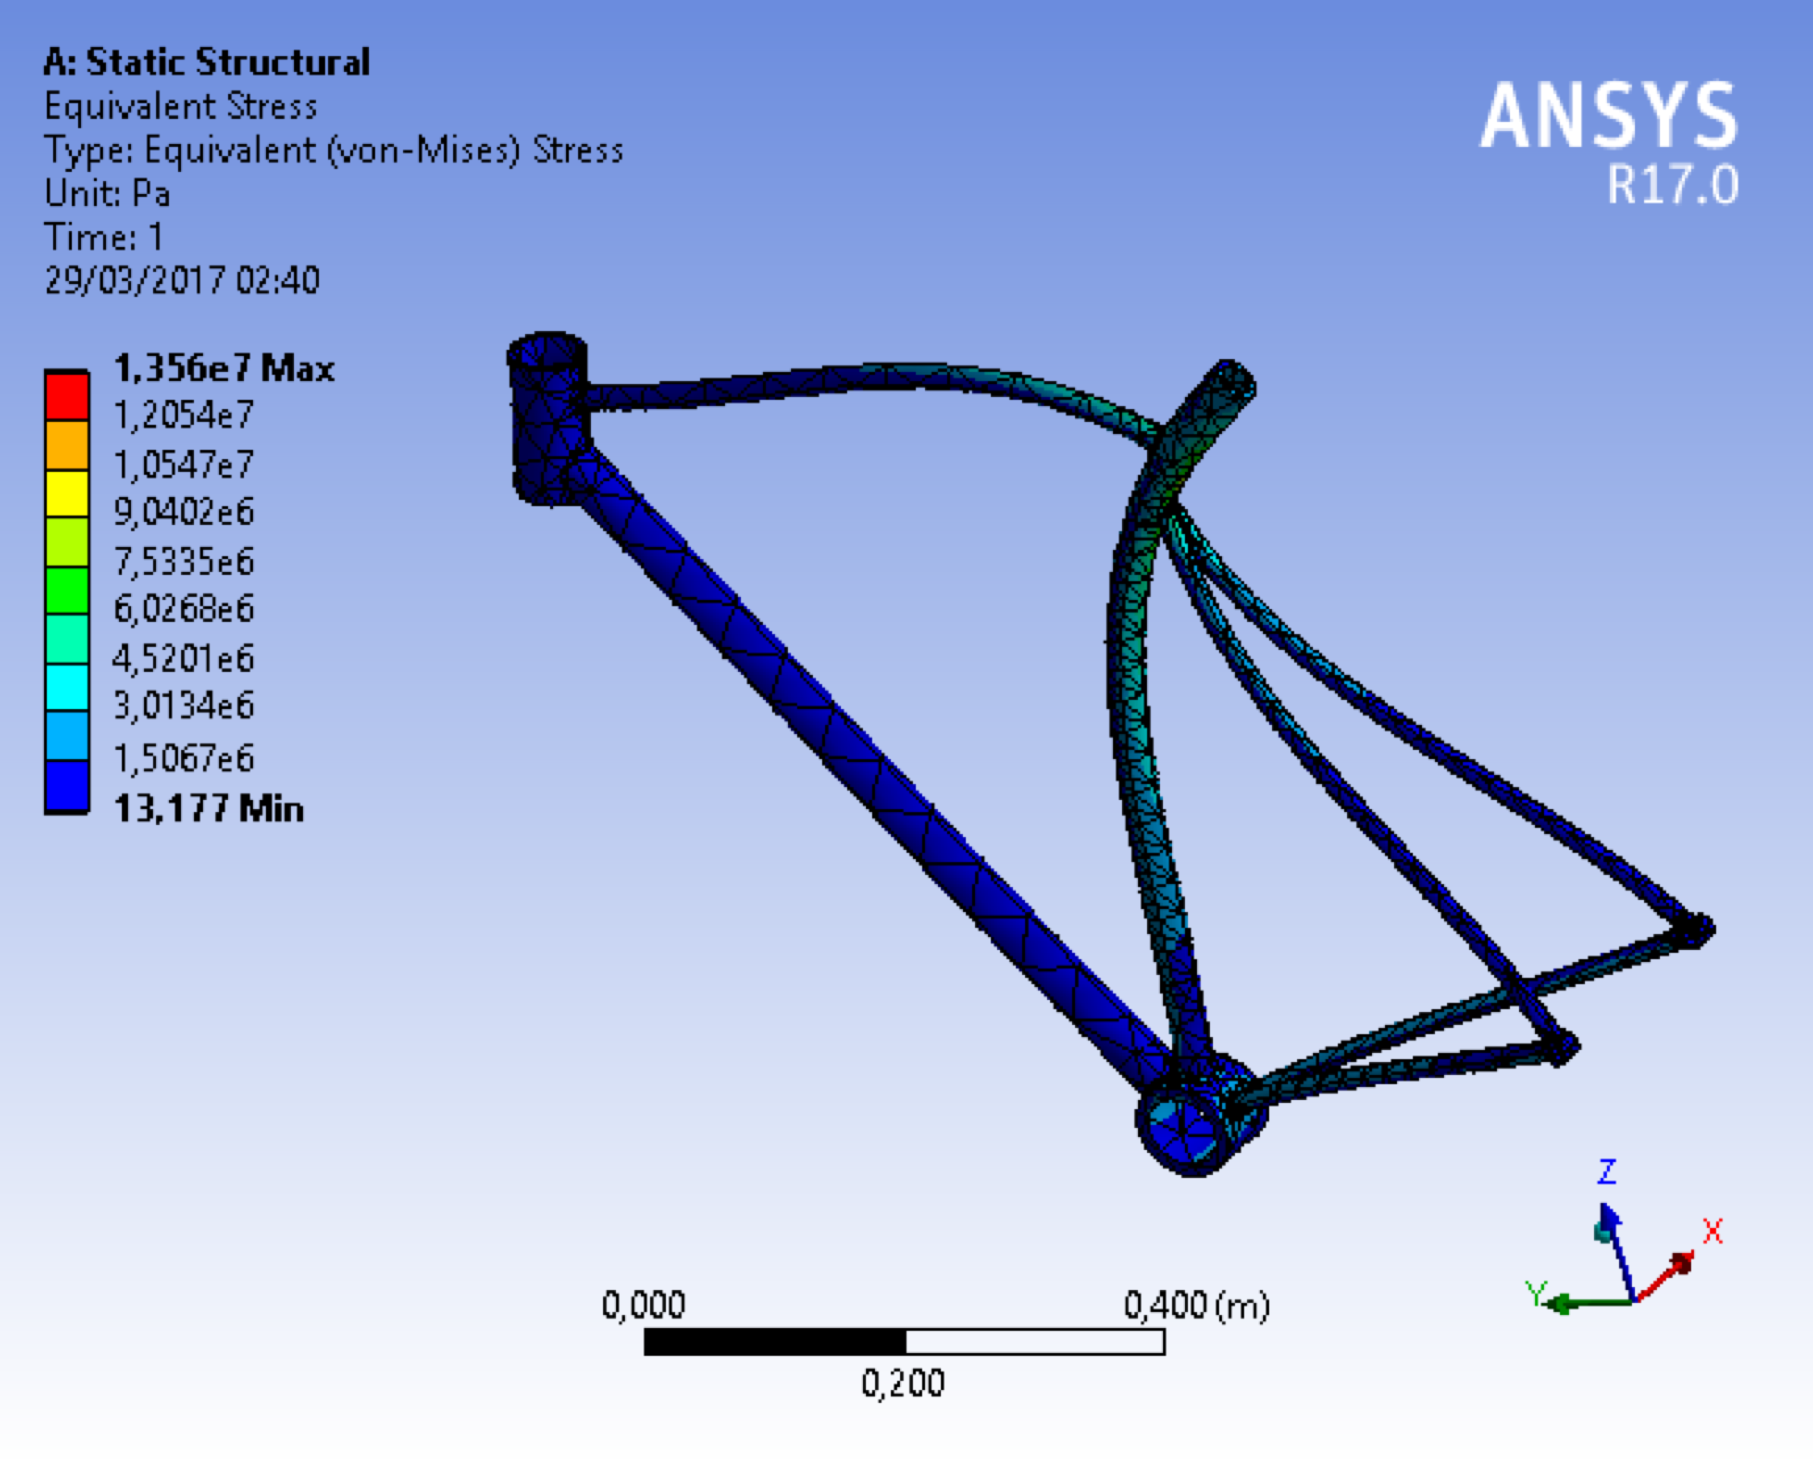
\includegraphics[scale=0.80]{equivalente_de_von_mises.png}
	\caption{Equivalente de von Mises}
	\label{img:equivalente_de_von_mises}
	\end{figure}	
	
\graphicspath{{figuras/}}
	\begin{figure}[h!]
	\centering
	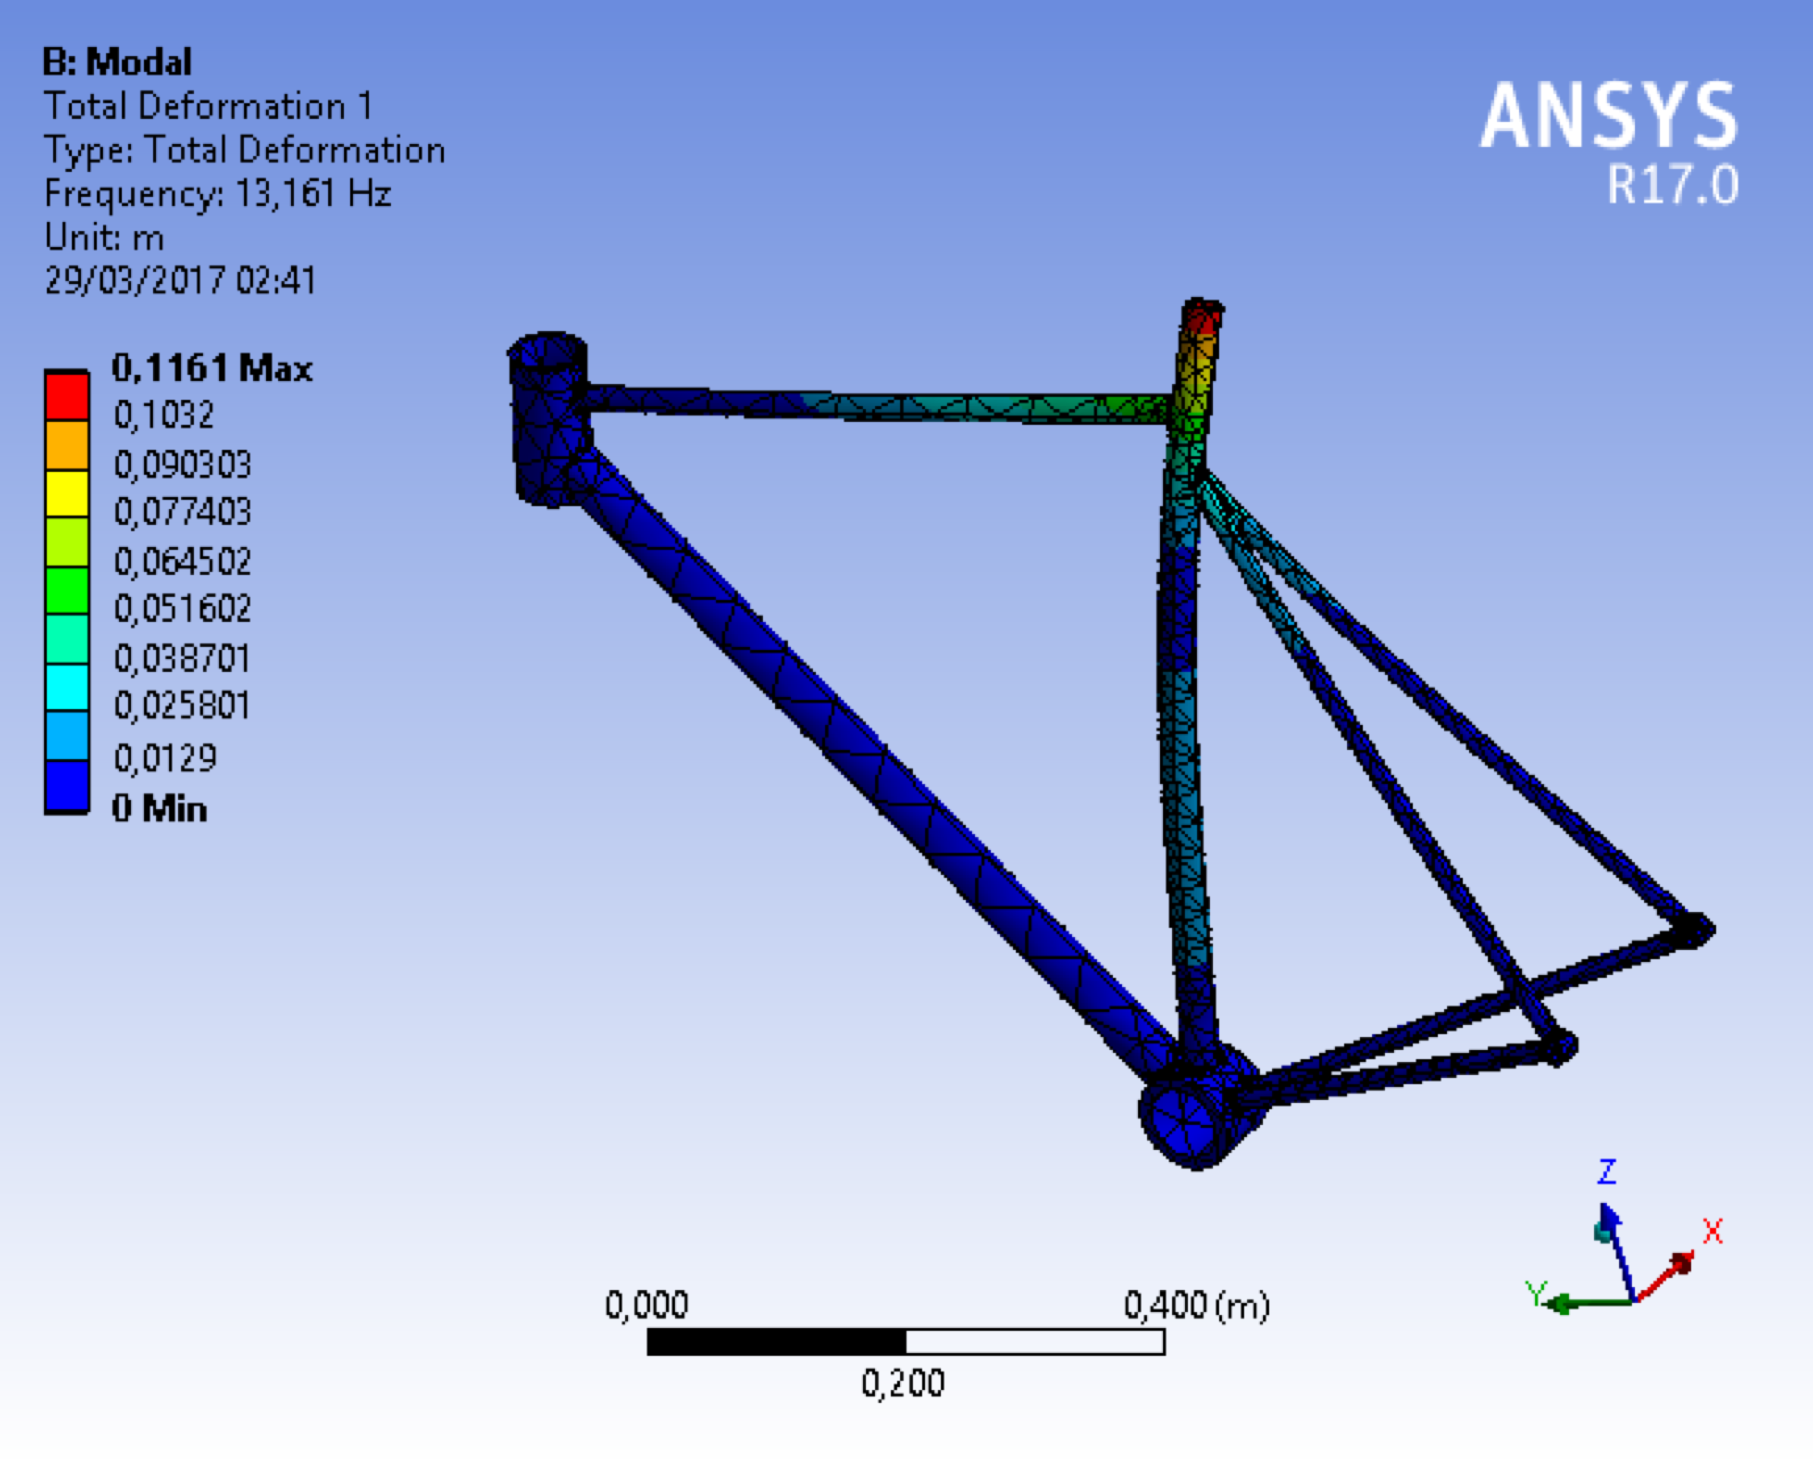
\includegraphics[scale=0.80]{modo_de_vibracao.png}
	\caption{Modo de vibracao}
	\label{img:modo_de_vibracao}
	\end{figure}	
	
\graphicspath{{figuras/}}
	\begin{figure}[h!]
	\centering
	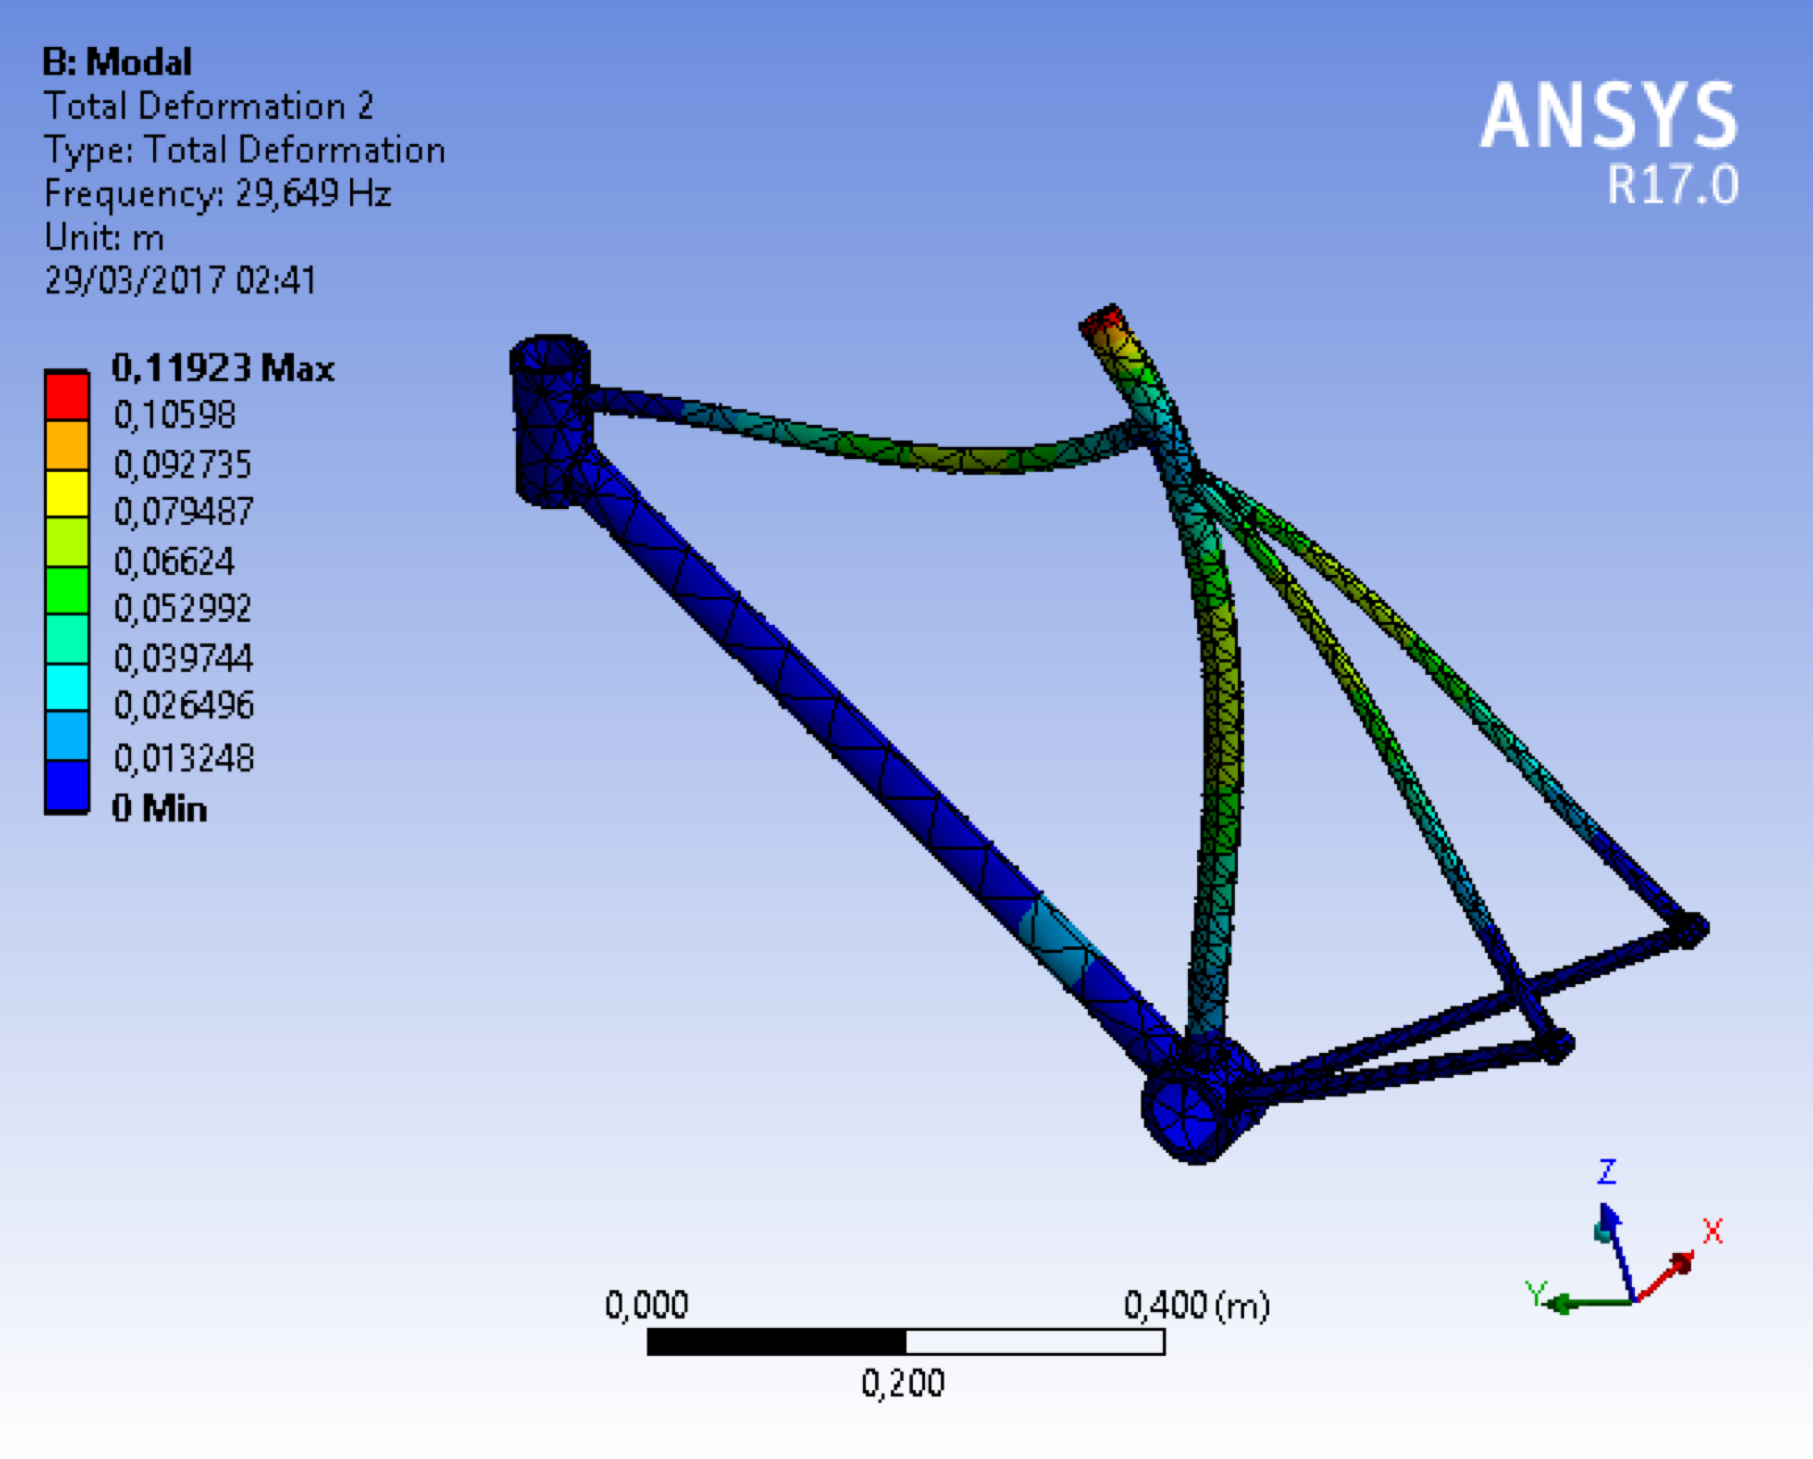
\includegraphics[scale=0.80]{modo_de_vibracao_2.png}
	\caption{Modo de vibracao 2}
	\label{img:modo_de_vibracao2}
	\end{figure}	
	
\graphicspath{{figuras/}}
	\begin{figure}[h!]
	\centering
	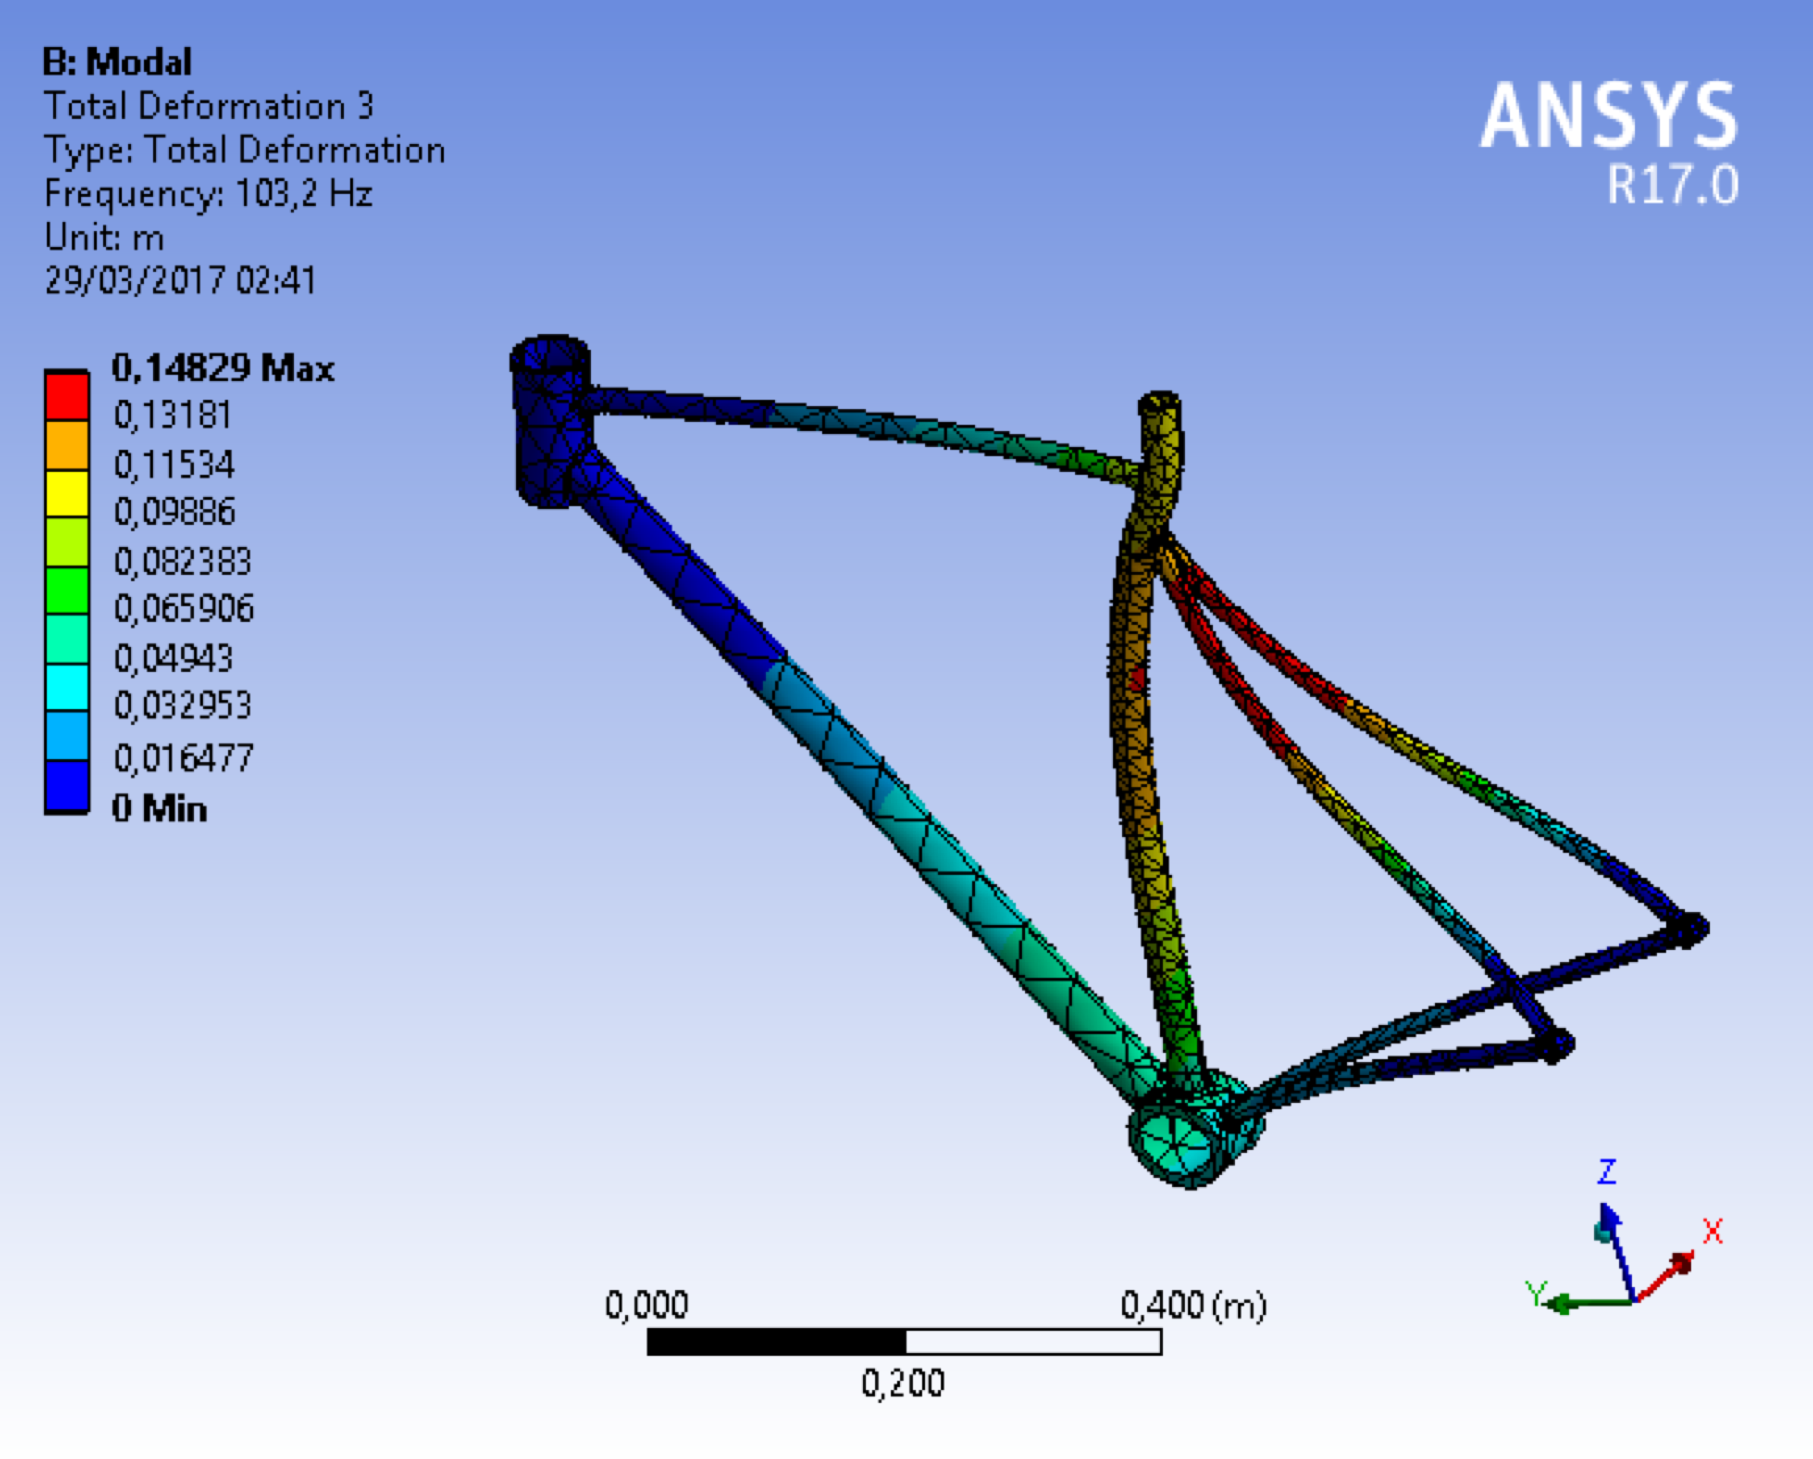
\includegraphics[scale=0.80]{modo_de_vibracao_3.png}
	\caption{Modo de vibracao 3}
	\label{img:modo_de_vibracao3}
	\end{figure}	
	
\graphicspath{{figuras/}}
	\begin{figure}[h!]
	\centering
	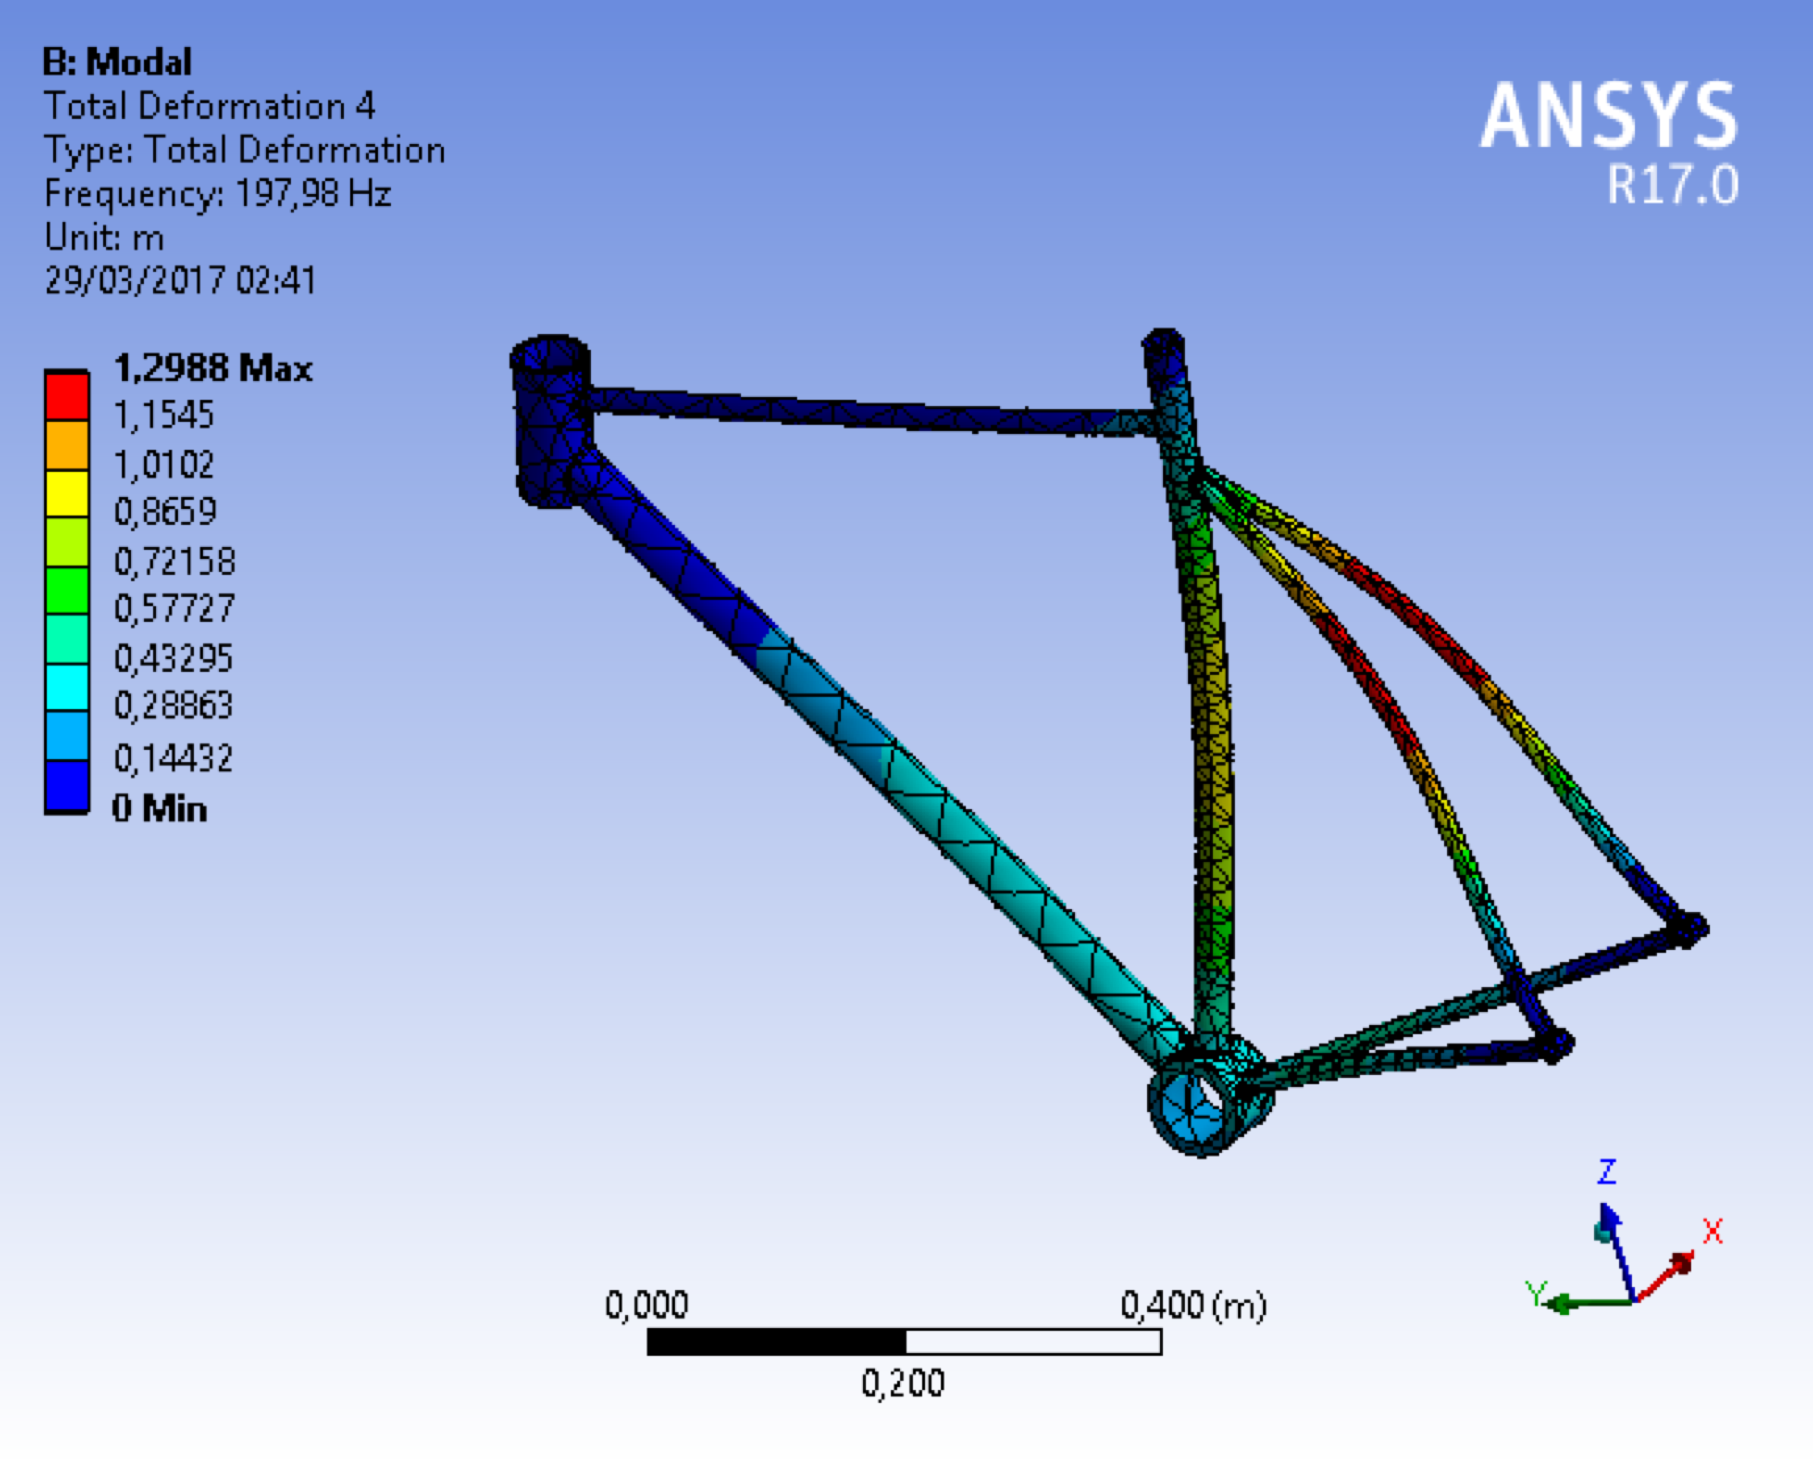
\includegraphics[scale=0.80]{modo_de_vibracao_4.png}
	\caption{Modo de vibracao 4}
	\label{img:modo_de_vibracao4}
	\end{figure}	
	
\graphicspath{{figuras/}}
	\begin{figure}[h!]
	\centering
	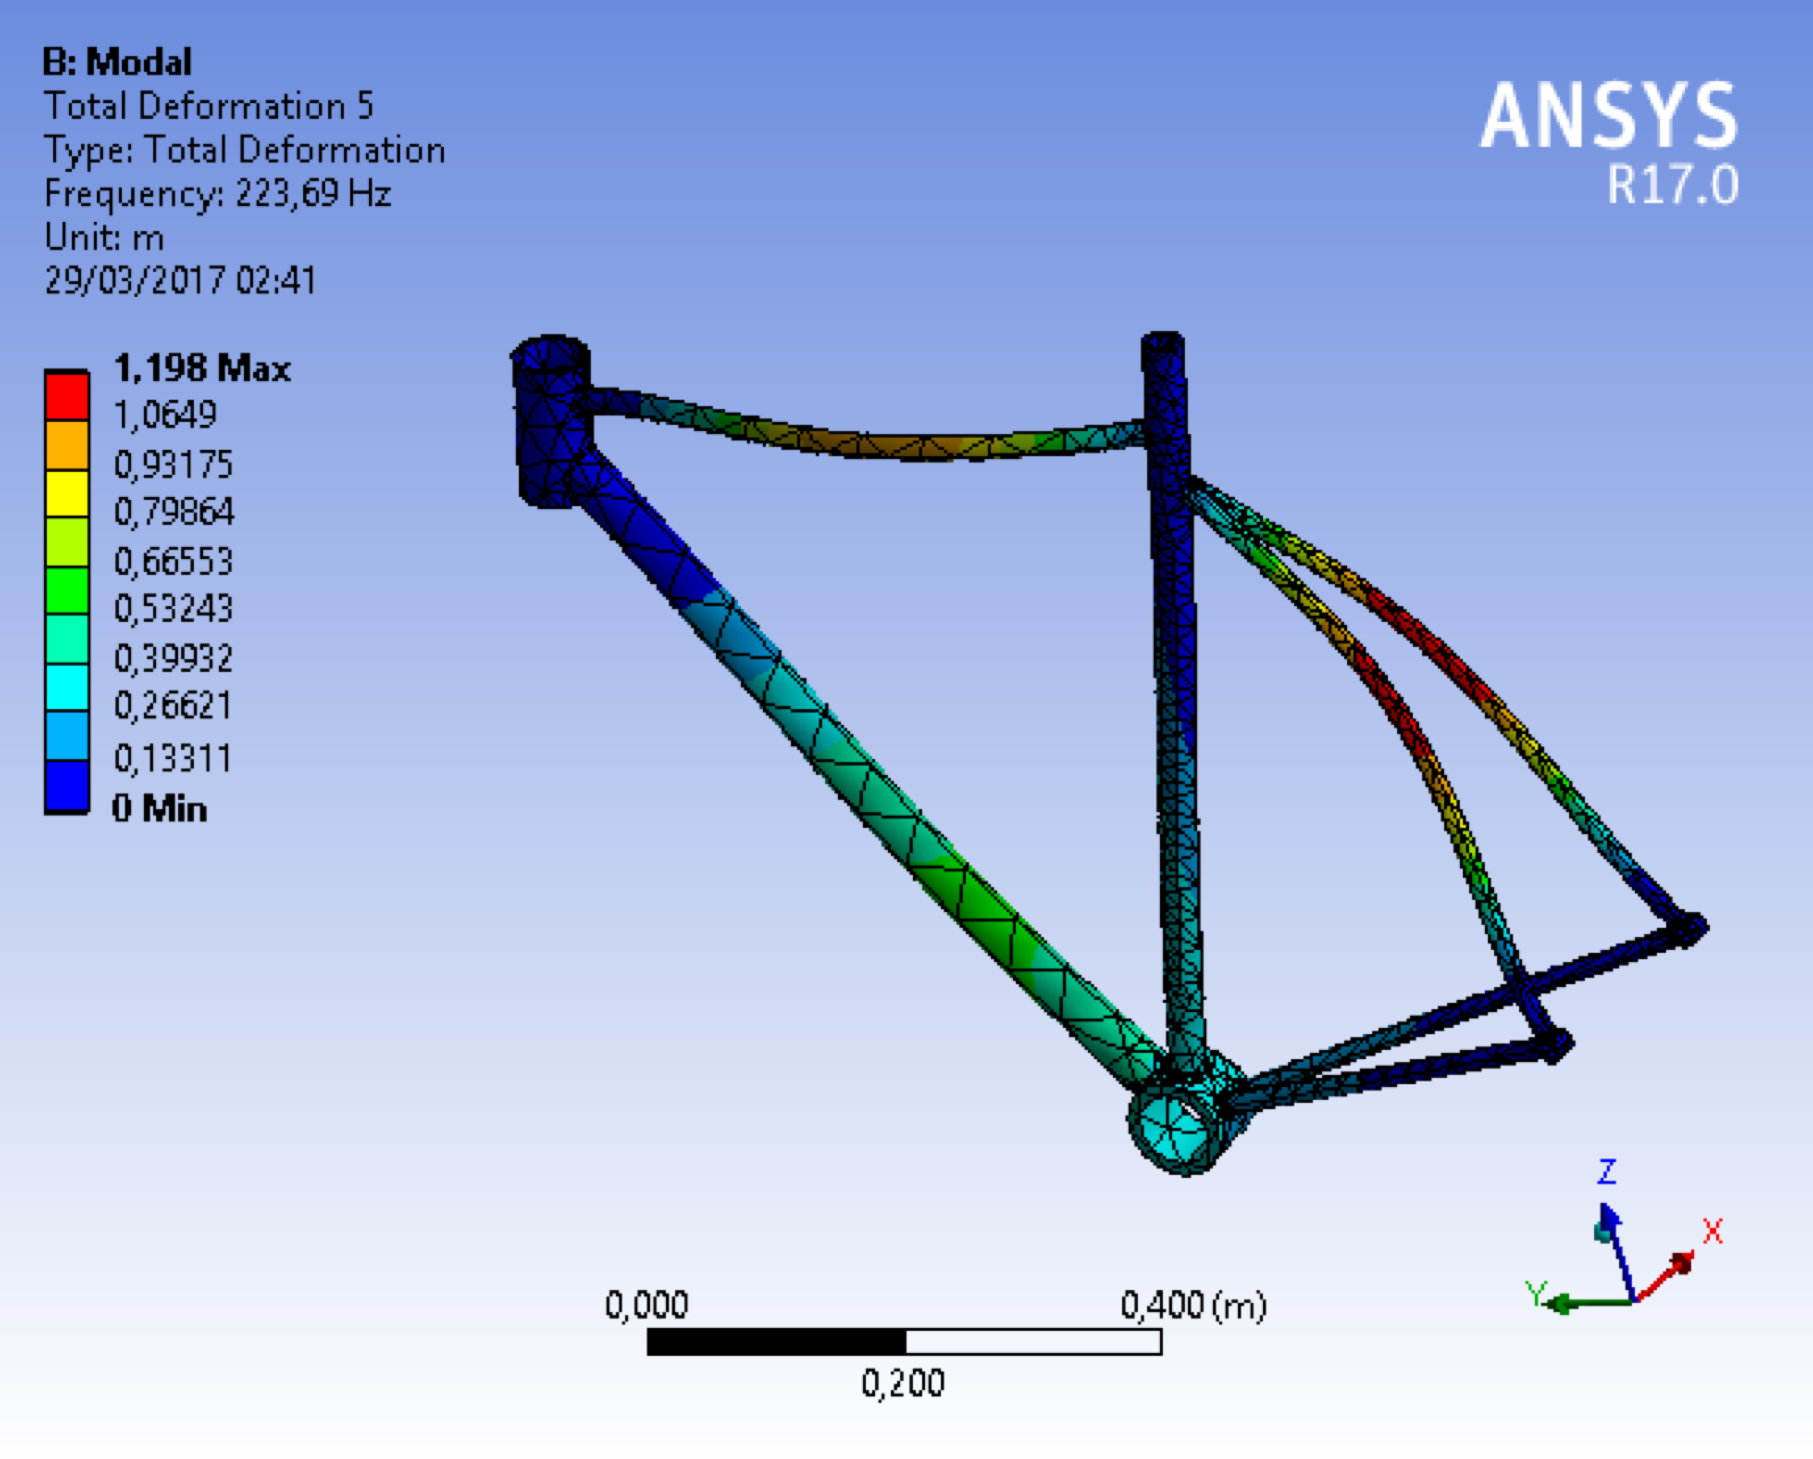
\includegraphics[scale=0.80]{modo_de_vibracao_5.png}
	\caption{Modo de vibracao 5}
	\label{img:modo_de_vibracao5}
	\end{figure}	

\graphicspath{{figuras/}}
	\begin{figure}[h!]
	\centering
	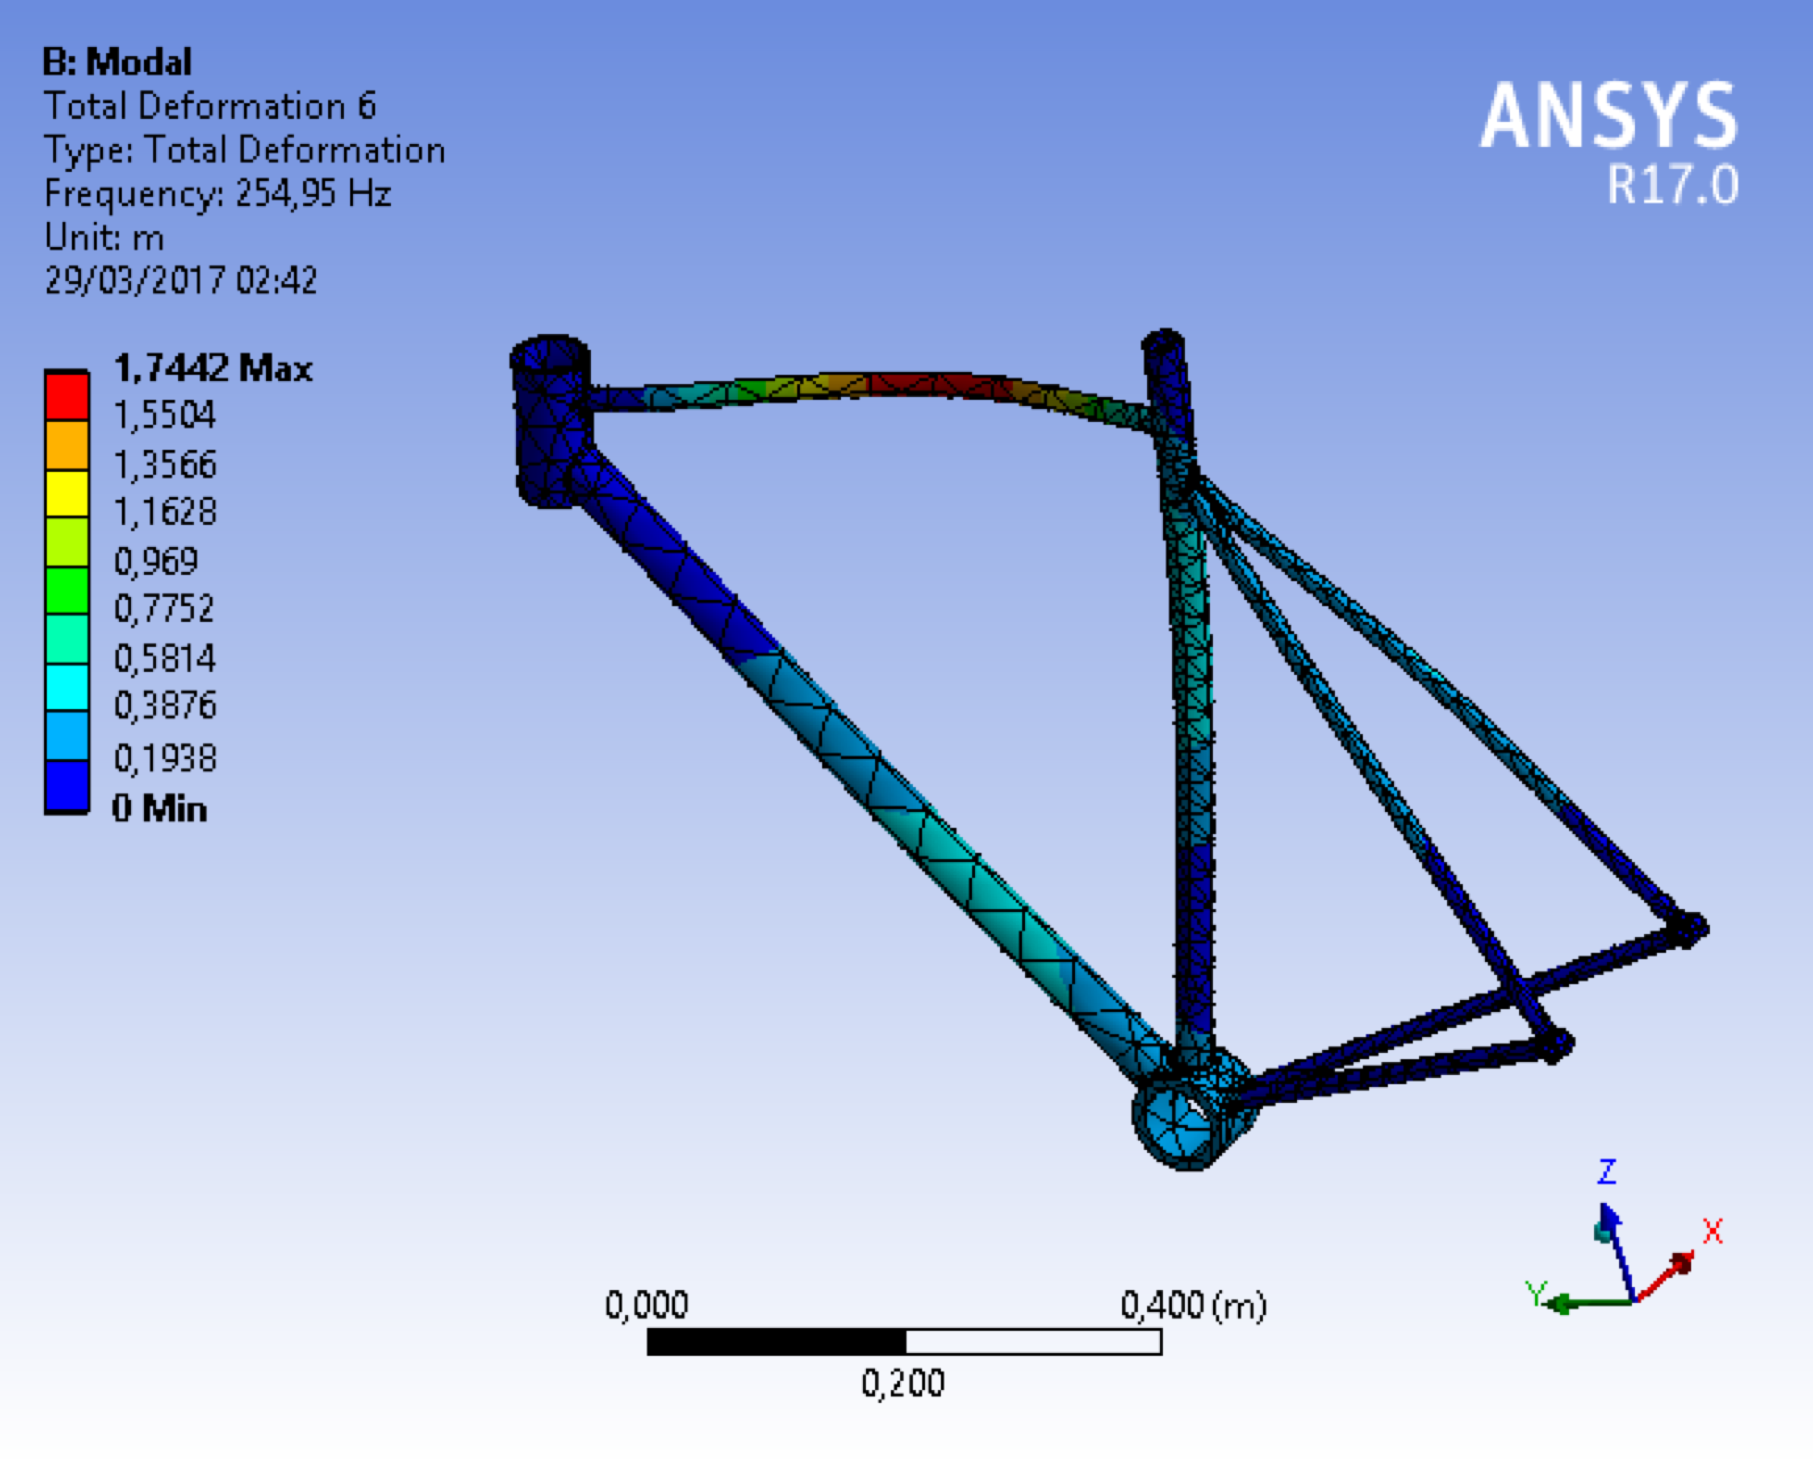
\includegraphics[scale=0.80]{modo_de_vibracao_6.png}
	\caption{Modo de vibracao 6}
	\label{img:modo_de_vibracao 6}
	\end{figure}	



	
	
	
	\subsection{Desafios Técnicos}
	Desafio: Definir uma geometria que comporte todo o sistema sem afetar a ergonomia do ciclista, e que seja capaz de suportar todas as solicitações mecânicas
Alternativa de solução: Alterar a geometria e/ou alterar o material da estrutura.

Desafio: impossibilidade de fabricação do quadro  por escassez de recursos, tempo ou incapacidade técnica.
Alternativa de solução: adquirir um quadro comum no comércio e realizar as adaptações necessárias

  \section{Normas}
  